\documentclass[tikz,border=6pt]{standalone}

\usepackage[T1]{fontenc}
\usepackage[utf8]{inputenc}
\usepackage{helvet}
\renewcommand{\familydefault}{\sfdefault}
\usepackage{amsmath}
\usepackage{tikz}
\usetikzlibrary{arrows.meta,positioning,fit,backgrounds,calc}

\definecolor{localblue}{HTML}{4E79A7}
\definecolor{timingorange}{HTML}{F28E2B}
\definecolor{lockgreen}{HTML}{59A14F}
\definecolor{consumerpurple}{HTML}{B07AA1}
\definecolor{softgray}{HTML}{F4F4F4}
\definecolor{linegray}{HTML}{5A5A5A}

\tikzset{
  block/.style={
    draw=linegray,
    rounded corners=3pt,
    thick,
    minimum width=3.35cm,
    minimum height=1.15cm,
    align=center,
    font=\sffamily\small,
    fill=white
  },
  subblock/.style={
    draw=linegray,
    rounded corners=2pt,
    semithick,
    minimum width=2.7cm,
    minimum height=0.82cm,
    align=center,
    font=\sffamily\scriptsize,
    fill=white
  },
  flow/.style={-{Latex[length=2.4mm]}, thick, draw=linegray},
  status/.style={-{Latex[length=2.1mm]}, semithick, dashed, draw=lockgreen!70!black},
  note/.style={font=\sffamily\scriptsize, text=linegray, align=center}
}

\begin{document}
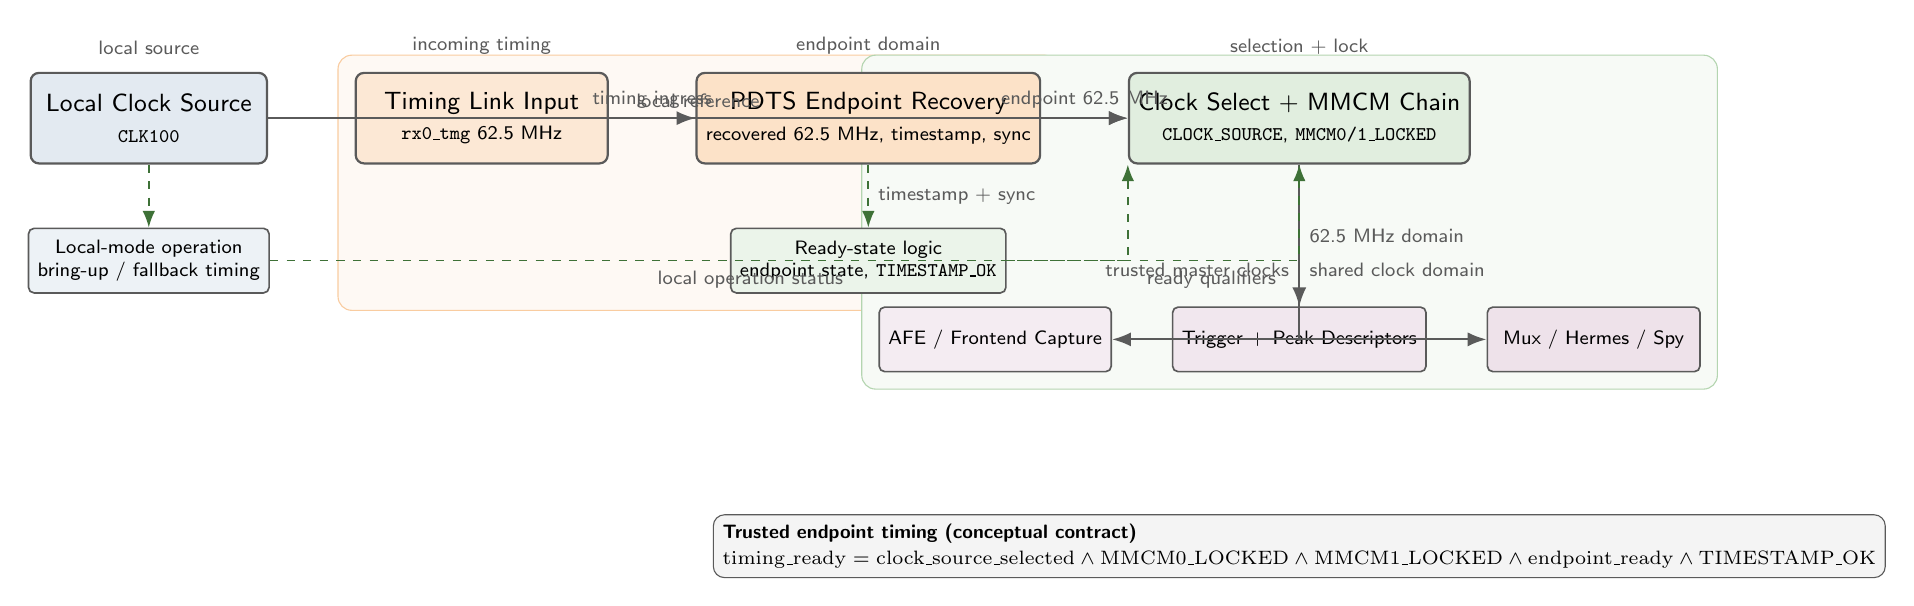
\begin{tikzpicture}[node distance=8mm and 11mm]

\node[block, fill=localblue!16, minimum width=3.0cm] (clk100) {Local Clock Source\\\scriptsize \texttt{CLK100}};
\node[block, fill=timingorange!20, right=of clk100, minimum width=3.2cm] (rxclk) {Timing Link Input\\\scriptsize \texttt{rx0\_tmg} 62.5 MHz};
\node[block, fill=timingorange!26, right=of rxclk, minimum width=3.7cm] (endpoint) {PDTS Endpoint Recovery\\\scriptsize recovered 62.5 MHz, timestamp, sync};
\node[block, fill=lockgreen!18, right=of endpoint, minimum width=4.0cm] (sel) {Clock Select + MMCM Chain\\\scriptsize \texttt{CLOCK\_SOURCE}, \texttt{MMCM0/1\_LOCKED}};

\node[subblock, fill=consumerpurple!14, below left=18mm and 2mm of sel] (frontend) {AFE / Frontend Capture};
\node[subblock, fill=consumerpurple!18, below=18mm of sel] (trigger) {Trigger + Peak Descriptors};
\node[subblock, fill=consumerpurple!22, below right=18mm and 2mm of sel] (transport) {Mux / Hermes / Spy};

\node[subblock, fill=lockgreen!12, below=of endpoint] (status) {Ready-state logic\\\scriptsize endpoint state, \texttt{TIMESTAMP\_OK}};
\node[subblock, fill=localblue!10, below=of clk100] (localmode) {Local-mode operation\\\scriptsize bring-up / fallback timing};

\begin{pgfonlayer}{background}
  \node[draw=timingorange!45, rounded corners=5pt, fill=timingorange!5,
        fit=(rxclk)(endpoint)(status), inner sep=6pt] {};
  \node[draw=lockgreen!45, rounded corners=5pt, fill=lockgreen!5,
        fit=(sel)(frontend)(trigger)(transport), inner sep=6pt] {};
\end{pgfonlayer}

% Clock flow
\draw[flow] (clk100) -- node[note, above] {local reference} (sel);
\draw[flow] (rxclk) -- node[note, above] {timing ingress} (endpoint);
\draw[flow] (endpoint) -- node[note, above] {endpoint 62.5 MHz} (sel);
\draw[flow] (sel) |- node[note, pos=0.30, left] {trusted master clocks} (frontend);
\draw[flow] (sel) -- node[note, right] {62.5 MHz domain} (trigger);
\draw[flow] (sel) |- node[note, pos=0.30, right] {shared clock domain} (transport);

% Status / readiness flow
\draw[status] (endpoint.south) -- node[note, right] {timestamp + sync} (status.north);
\draw[status] (status.east) -| node[note, pos=0.35, below] {ready qualifiers} (sel.south);
\draw[status] (localmode.east) -| node[note, pos=0.28, below] {local operation status} (sel.south west);
\draw[status] (clk100.south) -- (localmode.north);

% Equation / conditions
\node[draw=linegray, rounded corners=4pt, fill=softgray, align=left,
      font=\sffamily\scriptsize, below=18mm of trigger, minimum width=10.5cm] (eq) {
\textbf{Trusted endpoint timing (conceptual contract)}\\[0.5mm]
\(
\mathrm{timing\_ready} =
\mathrm{clock\_source\_selected}
\land
\mathrm{MMCM0\_LOCKED}
\land
\mathrm{MMCM1\_LOCKED}
\land
\mathrm{endpoint\_ready}
\land
\mathrm{TIMESTAMP\_OK}
\)
};

\node[note, above=1mm of clk100] {local source};
\node[note, above=1mm of rxclk] {incoming timing};
\node[note, above=1mm of endpoint] {endpoint domain};
\node[note, above=1mm of sel] {selection + lock};

\end{tikzpicture}
\end{document}
